La smart Gateway présente un rôle central dans notre architecture, c’est elle qui va faire l’intermédiaire entre les parties plus bas niveau comprenant les dispositifs et le middleware s’occupant de gérer ces dispositifs, et la partie supérieure qui correspond au reste de l’application avec le stockage des données, et les différentes applications. La Figure \ref{gateway} illustre le middleware que nous avons adopté au niveau du Gateway.
\newline
\begin{figure}[h!]
	\hspace*{-3cm}
	\centering
	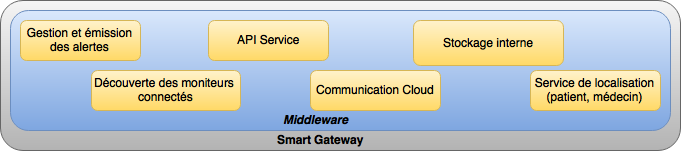
\includegraphics[width=1.5\textwidth]{Figure6.png}
	\caption{Middleware au niveau du Gateway}
	\label{gateway}
\end{figure}

Dans notre cas, elle va avoir différents modules pour répondre aux exigences du système. Elle aura un rôle primordial dans la transmission en temps réel des alertes depuis les couches inférieures, pour cela, un module autonome de gestion et d’émission des alertes sera présent pour pouvoir recevoir et réémettre aux bons destinataires ou aux bonnes applications les alertes, ce module pourra être couplé avec un module de localisation du personnel médical et du patient, pour que l’alerte soit déclenchée dans la zone proche du patient et qu’elle atteigne le personnel médicale compétent pour agir sur cette urgence tout en leur signalant la localisation de l’urgence. Ce module aura besoin d’être fiable et disponible dans la gestion des événements qu’elle reçoit car ceux-ci peuvent être des alertes vitales sur des patients.

L’identification des patients, et leur localisation dans l’hôpital est une nécessité, la présence d’un module permettant d’ajouter au réseau les nouveaux moniteurs connectés est indispensable. Dans l’architecture que nous proposons, nous avons un module dédié à la recherche des appareils, qui dans ce middleware sera la recherche des moniteurs intelligents. Les appareils de plus bas niveau vont se déclarer à ceux de plus haut niveau pour que ces derniers puissent les identifier de manière unique et leur associer les bonnes informations. Dans notre cas par exemple, lors de l’installation d’un nouveau patient, le moniteur va rechercher ou recevoir l’identifiant du patient, et une fois connectée au réseau, il se déclarera auprès de la passerelle intelligente la plus proche pour que celle-ci puisse mettre en mémoire la correspondance entre le moniteur et le patient. Une fois l’élément entré dans la table de correspondance de la passerelle intelligente, toutes les informations fournies par le moniteur pourront être transmises de manière cohérente auprès de la passerelle qui fera la redirection pour le stockage ou l’interprétation des données. Et la passerelle intelligente, informera ensuite le serveur IoT et les autres passerelles de la présence de ce nouvel élément. La méthode de recherche des dispositifs que nous proposons permettra une évolutivité et une adaptabilité aisées du système.

Une fois qu’une passerelle intelligente a pris connaissances des moniteurs connectés dans sa zone de couverture, elle va avoir pour rôle de transmettre les différentes informations de ces moniteurs pour leur stockage. Elle va donc s’occuper de gérer les données reçues avec l’aide d’un module de communication Cloud, qui s’occupera de faire l’intermédiaire entre les couches de stockage et les couches supérieures, pour cela elle doit être capable de communiquer avec les moyens de stockages que nous proposons sous forme de Cloud. Ce module s’occupera donc de la gestion des données, et sera donc couplé avec un module de stockage interne, qui servira de table de correspondances entre les différents moniteurs intelligents et le patient auquel il réfère. Le module de stockage interne servira à avoir le contexte des données qui sont fournies.

Comme nous avons pu le voir jusqu’à maintenant, le middleware présent au niveau du smart gateway a un rôle primordial dans le traitement et la redirection des informations, il doit être capable de faire ces différentes tâches en prenant en compte la sécurité des données qui transitent. La smart gateway va avoir un module d’authentification et de contrôle d’accès pour restreindre l’accès à ces données et éviter le vol de données privées sur les patients. Les applications dans le domaine de la santé, recueillent des informations confidentielles sur les patients, l’exposition de ces informations peut avoir des conséquences sur la vie privée et professionnelle de ces personnes, c’est pourquoi nous incorporons différents modules de sécurité dans les différentes couches de notre système. La smartGateway va ainsi posséder un module de chiffrement des communications pour garder la confidentialité des données qui sont transmises. Le couplage de ce module avec un module d’authentification et de contrôle d’accès va nous permettre d’avoir des mesures de sécurité quant aux informations des patients.

Enfin pour l’évolutivité du système proposé ainsi que l’ajout de différentes fonctionnalités, nous proposons un module API service qui contiendra les différentes API nécessaire à la transcription de méthodes et d’application depuis d’autres plateformes, il sera ainsi facile d’ajouter des fonctionnalités à la smart gateway comme par exemple l’introduction de nouveaux capteurs, et nous aurons donc une abstraction du code qui permettra une intégration plus facile de nouveaux éléments.
